\documentclass[times, utf8, seminar, numeric]{fer}
\usepackage{booktabs}
\usepackage{float}
\usepackage{footmisc}

\begin{document}

% TODO: Navedite naslov rada.
\title{Fast sequence alignment}

% TODO: Navedite vaše ime i prezime.
\author{Kristijan Biščanić \\ Luka Hrabar \\ Ela Marušić}

\maketitle

\tableofcontents

\chapter{Introduction}
This project will implement, test and analyse a faster algorithm for computing string edit distances and sequence alignment. This algorithm was published by Masek and Paterson \cite{masek1980faster} and is inspired by the Four Russians Algorithm. Implemented algorithm will be compared to and tested against Needleman-Wunsch algorithm \cite{needleman1970general}, which is based on dynamic programming.

The \textit{string edit distance} is defined as the minimal cost of transforming one character string into the other. Operations allowed in those transformations are only insertion, deletion and replacing of one character, each of these having defined some cost. \textit{Edit Script} is defined as the actual sequence of operations used to transform one string into the other. There are many algorithms that are using string edit distances and edit scripts for further calculations, and they are used extensively in bioinformatics for sequence alignment.

Sequence alignment is a process of arranging the symbolic representations of DNA, RNA or protein sequences so that their most similar elements are juxtaposed. Such alignment is useful to identify regions of similarity and many bioinformatics tasks depend upon successful alignments.

\chapter{Algorithm}
\section{The basic algorithm}
Dynamic programming problems can, most often than not, be reduced to a matrix of solutions to subproblems where the value of a cell ($i$, $j$) depends only on the cells with coordinates ($u\leq i$, $v\leq j$). This is the case with the edit distance and string alignment problems. An example is shown in table \ref{tab:a}, with the final solution in cell ($N$, $M$).
\begin{table}[H]
\centering
\begin{tabular}{c|ccccc}
  & - & G & C & A & T\\
\hline
- & $0$ & $1$ & $2$ & $3$ & $4$ \\
G & $1$ & $\cdot$ & $\cdot$ & $\cdot$ & $\cdot$ \\
A & $2$ & $\cdot$ & $\cdot$ & $\cdot$ & $\cdot$ \\
T & $3$ & $\cdot$ & $\cdot$ & $\cdot$ & $\cdot$ \\
T & $4$ & $\cdot$ & $\cdot$ & $\cdot$ & $\cdot$ \\
\end{tabular}
\quad\quad
\begin{tabular}{c|ccccc}
  & - & G & C & A & T\\
\hline
- & $0$ & $1$ & $2$ & $3$ & $4$ \\
G & $1$ & $0$ & $1$ & $2$ & $3$ \\
A & $2$ & $1$ & $2$ & $1$ & $2$ \\
T & $3$ & $2$ & $3$ & $2$ & $1$ \\
T & $4$ & $3$ & $4$ & $3$ & $2$ \\
\end{tabular}
\caption{String edit matrix $E$}\label{tab:a}
\end{table}

The first row and column of the matrix are computed using the operation costs for the corresponding character. All other values in the matrix are computed as:
\begin{equation}
E_{i,j} = min(E_{i-1, j-1} + R, E_{i-1, j} + I, E_{i, j - 1} + D)
\end{equation}
where $R$, $I$, $D$ are the costs of the (matrix movement) operations described in the introduction.
Due to the fact that each value can be computed in $O(1)$ time in the presented manner, both the time and space complexities of this matrix calculation equal $O(N \times M)$, where $N$ and $M$ denote the length of the strings.

\section{The basic algorithm with optimized space complexity}
Lets say we traverse and fill the matrix from earlier in a row-major fashion. If we take a closer look we'll notice that the values from row $i$ depend only on the values from the previous row, $i-1$, and on the values we've already calculated in this row. Therefore, we can forget the values from row $i-2$ and earlier, effectively reducing the memory required for the algorithm to two arrays of length equal to the number of columns. In other terms, the space complexity is reduced to $O(min(N, M))$ if we set the determine the number of columns using the shorter of the two strings in question.

\section{The Four Russians method}
We know that a problem matrix is represented using two strings and two initial vectors of values as shown earlier. In fact, every subproblem of our problem is represented using such strings and vectors:

\begin{figure}[H]
\centering
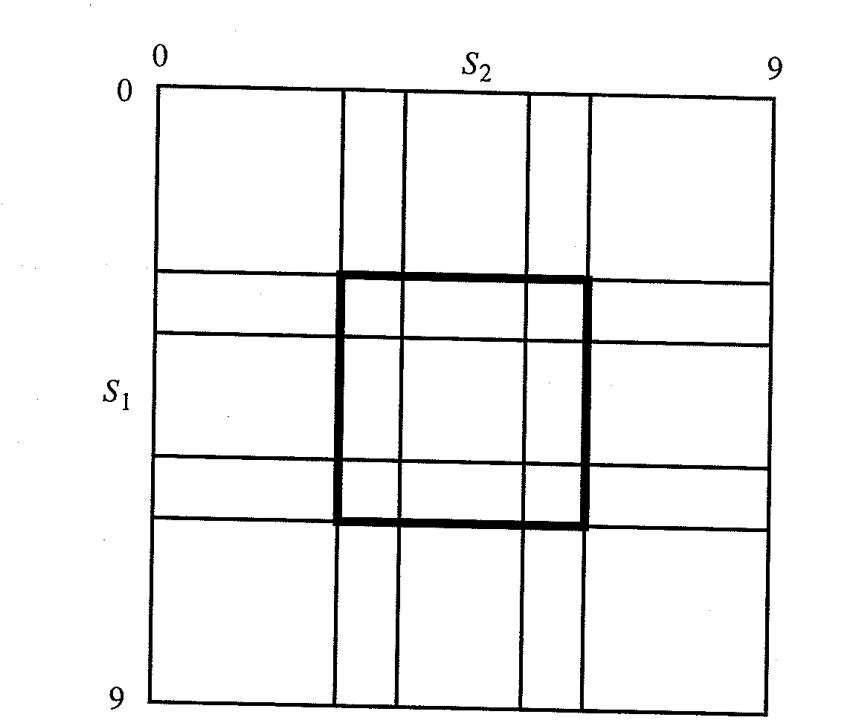
\includegraphics[scale=.25]{s1}
\caption{Submatrices}\label{pic:s1}
\end{figure}

If we split the matrix into smaller submatrices (\ref{pic:s1}) and precalculate the solutions of these subproblems we can combine them to solve the large matrix. This is possible because the final vectors of some submatrix are the initial vectors of some other submatrices as seen in (\ref{pic:s1}). The final solution is yet again in the bottom-right cell of the large matrix.

The space and time complexities using this technique would be reduced to \\
$O(min(N, M) / t)$ and $O(N * M / t^2)$, respectively. The $t$ denotes the dimension of the submatrices used. But, in order for it to work, we need to precalculate every submatrix that might occur in our problem.

\section{Precalculating the submatrices}
The number of initial submatrix setup combinations is determined using the following expression:
\begin{equation}
  combinations = |\sigma|^2t \cdot |\lambda|^2t
\end{equation}
The expression is derived from the fact that every subproblem is determined using two initial vectors of costs and two strings. $|\sigma|$ denotes the size of the alphabet used for the strings, $t$ represents the submatrix dimension, and $|\lambda|$ is the size of the set that contains every value that can occur in the initial vectors.

\section{The step observation}
The set of possible values from earlier can obviously be pretty large and we need to find a way to reduce the number of precalculations. Fortunately, we have the following observation - the values in these initial vectors, i.e. the values in general, tend to increase as we move towards the bottom-right corner of the matrix.

Before we continue, we will fix the operation costs as follows, in the context of string alignment:
\begin{itemize}
\item move right in the matrix, i.e. use the next character of the top string, will have cost $1$
\item move down in the matrix, i.e. use the next character of the left string, will have cost $1$
\item move diagonally down-right, i.e. use both strings' next characters will have cost $0$ if the characters match, $2$ otherwise
\end{itemize}
With these costs, the difference between any two adjacent matrix elements is restricted to \{$-1$, $0$, $1$\} (for proof see \citep{gusfield1997algorithms}).

The next step is to code all matrix values using these differences. We have two expressions, one for vertical steps and one for horizontal steps (for more details see \citep{masek1980faster}):
\begin{equation}
\delta_{i,j} - \delta_{i-1,j} = min\{R_{i,j} - (\delta_{i-1,j}-\delta_{i-1,j-1}), D, I + (\delta_{i,j-1} - \delta_{i-1, j-1})\}
\end{equation}
\begin{equation}
\delta_{i,j} - \delta_{i,j-1} = min\{R_{i,j} - (\delta_{i,j-1}-\delta_{i-1,j-1}), D + (\delta_{i-1,j} - \delta_{i-1, j-1}), I\}
\end{equation}

$D$ and $I$ are the the costs of deletion and insertion, which are $1$ in our case. $R_{i,j}$ denotes the cost of replacing the $i$-th character of the first string with the $j$-th character of the second and is equal to $0$ if the two characters match ($2$ otherwise).

We are now able to reduce the number of submatrices we have to precalculate using vectors of steps, one horizontal and one vertical, instead of vectors of matrix values to:
\begin{equation}
combinations = |\sigma|^2t \cdot 3^2t
\end{equation}

To save space we will be storing only the final vectors for each submatrix, mapped to the initial vector and string combination. The time complexity to calculate a single submatrix's final step vectors is $O(t^2)$.

\section{Combining everything}
Once we have computed all the possible submatrices, we can use them to generate the edit matrix of steps. More precisely, since we have two types of steps (those moving horizontally and those moving vertically), we will be generating two edit matrices of steps.

The first row and column of the matrix are initialized as demonstrated in the example below. The initial cost in the top left cell is 0, and the cells in the column and row are filled with the cost of deletion and insertion, respectively.

\begin{table}[H]
\centering
\begin{tabular}{c|ccccc}
  & - & G & C & A & T\\
\hline
- & $0$ & $1$ & $1$ & $1$ & $1$ \\
G & $\cdot$ & $\cdot$ & $\cdot$ & $\cdot$ & $\cdot$ \\
A & $\cdot$ & $\cdot$ & $\cdot$ & $\cdot$ & $\cdot$ \\
T & $\cdot$ & $\cdot$ & $\cdot$ & $\cdot$ & $\cdot$ \\
T & $\cdot$ & $\cdot$ & $\cdot$ & $\cdot$ & $\cdot$ \\
\end{tabular}
\quad\quad
\begin{tabular}{c|ccccc}
  & - & G & C & A & T\\
\hline
- & $0$ & $\cdot$ & $\cdot$ & $\cdot$ & $\cdot$ \\
G & $1$ & $\cdot$ & $\cdot$ & $\cdot$ & $\cdot$ \\
A & $1$ & $\cdot$ & $\cdot$ & $\cdot$ & $\cdot$ \\
T & $1$ & $\cdot$ & $\cdot$ & $\cdot$ & $\cdot$ \\
T & $1$ & $\cdot$ & $\cdot$ & $\cdot$ & $\cdot$ \\
\end{tabular}
\caption{Matrices of horizontal and vertical steps}
\end{table}

The rest of the matrix can now be filled with submatrices we have already calculated. We know the first row and column and the substrings for the top-left submatrix, so we can simply retrieve the precalculated final row and column.

\begin{table}[H]
\centering
\begin{tabular}{c|ccccc}
  & - & G & C & A & T\\
\hline
- & $0$ & $1$ & $1$ & $1$ & $1$ \\
G & $\cdot$ & $\cdot$ & $\cdot$ & $\cdot$ & $\cdot$ \\
A & $0$ & $-1$ & $1$ & $\cdot$ & $\cdot$ \\
T & $\cdot$ & $\cdot$ & $\cdot$ & $\cdot$ & $\cdot$ \\
T & $\cdot$ & $\cdot$ & $\cdot$ & $\cdot$ & $\cdot$ \\
\end{tabular}
\quad\quad
\begin{tabular}{c|ccccc}
  & - & G & C & A & T\\
\hline
- & $0$ & $\cdot$ & $0$ & $\cdot$ & $\cdot$ \\
G & $1$ & $\cdot$ & $-1$ & $\cdot$ & $\cdot$ \\
A & $1$ & $\cdot$ & $1$ & $\cdot$ & $\cdot$ \\
T & $1$ & $\cdot$ & $\cdot$ & $\cdot$ & $\cdot$ \\
T & $1$ & $\cdot$ & $\cdot$ & $\cdot$ & $\cdot$ \\
\end{tabular}
\end{table}

Since the submatrices in our matrix overlap, the last column of a submatrix is also the first column of the submatrix to the right (and the last row is also the first row of the submatrix below). Knowing this, we can continue to determine the last row and column of submatrices in a rowwise manner.

\begin{table}[H]
\centering
\begin{tabular}{c|ccccc}
  & - & G & C & A & T\\
\hline
- & $0$ & $1$ & $1$ & $1$ & $1$ \\
G & $\cdot$ & $\cdot$ & $\cdot$ & $\cdot$ & $\cdot$ \\
A & $0$ & $-1$ & $1$ & $-1$ & $1$ \\
T & $\cdot$ & $\cdot$ & $\cdot$ & $\cdot$ & $\cdot$ \\
T & $0$ & $-1$ & $1$ & $-1$ & $-1$ \\
\end{tabular}
\quad\quad
\begin{tabular}{c|ccccc}
  & - & G & C & A & T\\
\hline
- & $0$ & $\cdot$ & $0$ & $\cdot$ & $0$ \\
G & $1$ & $\cdot$ & $-1$ & $\cdot$ & $-1$ \\
A & $1$ & $\cdot$ & $1$ & $\cdot$ & $-1$ \\
T & $1$ & $\cdot$ & $1$ & $\cdot$ & $-1$ \\
T & $1$ & $\cdot$ & $1$ & $\cdot$ & $1$ \\
\end{tabular}
\end{table}

The edit distance is the sum of steps along some path from the top left cell to the bottom right. For example, if we sum the steps along the first column and the last row, we get an edit distance of $2$. The sequence of edit operations can be retrieved, provided that we have kept in memory all of the step rows and columns. We can now backtrack through the matrix by regenerating the submatrices which are crossed by the edit path. This is possible since the value in the top left cell of each submatrix can be computed in the same manner as the final edit distance, and the steps along the top row and left column are known.

\section{Complexity analysis}
If we set the submatrix dimension as $t = log_{3|\sigma|}N$, the total time complexity is equal to:
\begin{itemize}
\item $O(N \cdot log_{3|\sigma|}^2N)$ for submatrix precalculation
\item $O(N^2 / log_{3|\sigma|}N)$ for submatrix combination
\end{itemize}

The second complexity assumes the submatrices are stored in some tree-like fashion and it takes $O(log_{3|\sigma|}N)$ time to retrieve a submatrix. If submatrices were to be indexed (e.g. with a perfect hashing algorithm) and stored in an array the complexity would be reduced by a factor of $log_{3|\sigma|}N$. For more details see \citep{gusfield1997algorithms}.

\chapter{Test results}
Our algorithm was tested on synthetic sequences. Pairs of sequence reads were simulated using wgsim tool from reference chromosome of Escherichia coli bacteria, and then converted into FASTA file format which is used as an input file format. Output file format of our program was MAF (\textit{Multiple Alignment Format}) containing score, which is equal to string edit distance, and sequence alignment for algorithms that support it. 

Pairs of sequence reads were generated with lengths of 100, 200, 500, 1 000, 5 000, 10 000, 50 000, 100 000, 500 000 and 1 000 000 characters. Every pair was then tested on our algorithm, as well as Needleman-Wunsch algorithm for reference. Every test was timed and maximal memory usage was observed for each of the algorithms. Fischer-Wagner algorithm was tested on sequences up to 100 000 characters because of its large time complexity. Both algorithms were tested in same conditions on the same computer running inside Bio-Linux-8 virtual machine with access to 2 CPU cores and 4GB RAM.
\begin{table}[h]
\centering
\begin{tabular}{rccc}
$N$ & Fischer-Wagner & Masek-Paterson & Masek-Paterson (alignment)\\
\hline
$      100 $&$ 0.483$ ms&$ 8.751$ ms&$ 10.25$ ms \\
$      200 $&$ 1.633$ ms&$ 33.99$ ms&$ 35.24$ ms \\
$      500 $&$ 7.954$ ms&$ 146.04$ ms&$ 151.66$ ms\\
$    1 000 $&$ 44.34$ ms&$ 366.47$ ms&$ 511.02$ ms\\
$    5 000 $&$ 847.7$ ms&$ 6.07$ s&$ 10.70$ s\\
$   10 000 $&$ 3.253$ s&$ 24.27$ s&$ 39.83$ s\\
$   50 000 $&$ 79.94$ s&$ 549.104$ s&$ - $\footnotemark[2]\\
$  100 000 $&$ 331.6$ s&$ 2$ s&$ - $\footnotemark[2]\\
$  500 000 $&$ 2 - 3$ h \footnotemark[1] &$ 2s $&$ - $\footnotemark[2]\\
$1 000 000 $&$ 9 - 10$ h \footnotemark[1] &$ 2s $&$ - $\footnotemark[2]\\
\end{tabular}
\caption{Time comparison}
\end{table}
\begin{table}[h]
\centering
\begin{tabular}{rccc}
$N$ & Fischer-Wagner & Masek-Paterson & Masek-Paterson (alignment) \\
\hline
$      100 $&$ 1756$ KB &$ 1612$ KB &$ 1828$ KB \\
$      200 $&$ 1756$ KB &$ 7172$ KB &$ 7380$ KB \\
$      500 $&$ 1768$ KB &$ 7180$ KB &$ 8432$ KB \\
$    1 000 $&$ 1772$ KB &$ 7180$ KB &$ 11.86$ MB\\
$    5 000 $&$ 1836$ KB &$ 7224$ KB &$ 126.4$ MB\\
$   10 000 $&$ 1924$ KB &$ 7276$ KB &$ 484.7$ MB\\
$   50 000 $&$ 2464$ KB &$ 805.59$ MB&$ - $\footnotemark[2]\\
$  100 000 $&$ 3188$ KB &$ 2s $&$ - $\footnotemark[2]\\
$  500 000 $&$ 2 - 3$ h\footnotemark[1]&$ 2s $&$ - $\footnotemark[2]\\
$1 000 000 $&$ 9 - 10$ h\footnotemark[1]&$ 2s $&$ - $\footnotemark[2]\\
\end{tabular}
\caption{Maximal memory consumption comparison}
\end{table}
\footnote{estimated, too much time to execute}
\footnote{too much memory to execute}

\chapter{Conclusion}
We've presented an implementation of fast string alignment as described in \cite{masek1980faster}. Using the Four Russians algorithm combined with the proposed edit matrix reduction system we've achieved a significant improvement over the quadratic string alignment algorithm. In terms of time complexity, our implementation is faster by a factor of $log_{3|\sigma|}(N)$ where $|\sigma|$ denotes the alphabet size. When discussing space complexity, we use less memory (by the same factor) but the required memory is still a bottleneck when dealing with long strings. Nevertheless, an improvement is visible - we can calculate the edit script for strings up to a million length if provided with a supercomputer, and that was not the case for the quadratic algorithm.

The method we explored leaves barely any room for space complexity optimization. With that in mind, the next potential improvement would be to research and implement a more memory-efficient idea, for example \cite{kundeti2008extending}.

\bibliography{literatura}
\bibliographystyle{fer}

\nocite{*}
\end{document}
